\documentclass[tikz,border=10pt]{standalone}
\begin{document}
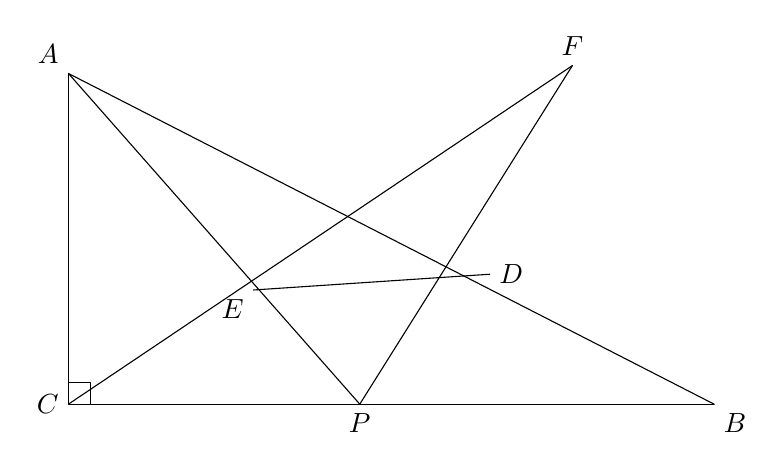
\begin{tikzpicture}[line cap=round,line join=round]

% Coordinates
\coordinate (C) at (0,0);
\coordinate (A) at (0,4.2);
\coordinate (B) at (8.2,0);
\coordinate (P) at (3.7,0);
\coordinate (F) at (6.4,4.3);
\coordinate (E) at (2.35,1.45);
\coordinate (D) at (5.35,1.65);

% Main edges
\draw (A) -- (C) -- (B);
\draw (A) -- (B);
\draw (C) -- (F);
\draw (A) -- (P);
\draw (P) -- (F);
\draw (E) -- (D);

% Right-angle mark at C
\draw (0,0.28) -- (0.28,0.28) -- (0.28,0);

% Labels
\node[above left] at (A) {$A$};
\node[left] at (C) {$C$};
\node[below right] at (B) {$B$};
\node[below] at (P) {$P$};
\node[above] at (F) {$F$};
\node[below left] at (E) {$E$};
\node[right] at (D) {$D$};

\end{tikzpicture}
\end{document}
